\documentclass{article}
\usepackage{main}

\title{Courbes représentatives}
\author{Seconde 9}
\date{06 Mars 2025}

\begin{document}
\maketitle

Soit $f, g$ et $h$ trois fonctions définies sur $\R$ dont les courbes représentatives $\mathcal{C}_f$, $\mathcal{C}_g$ et $\mathcal{C}_h$ sont représentées ci-contre.
\begin{center}
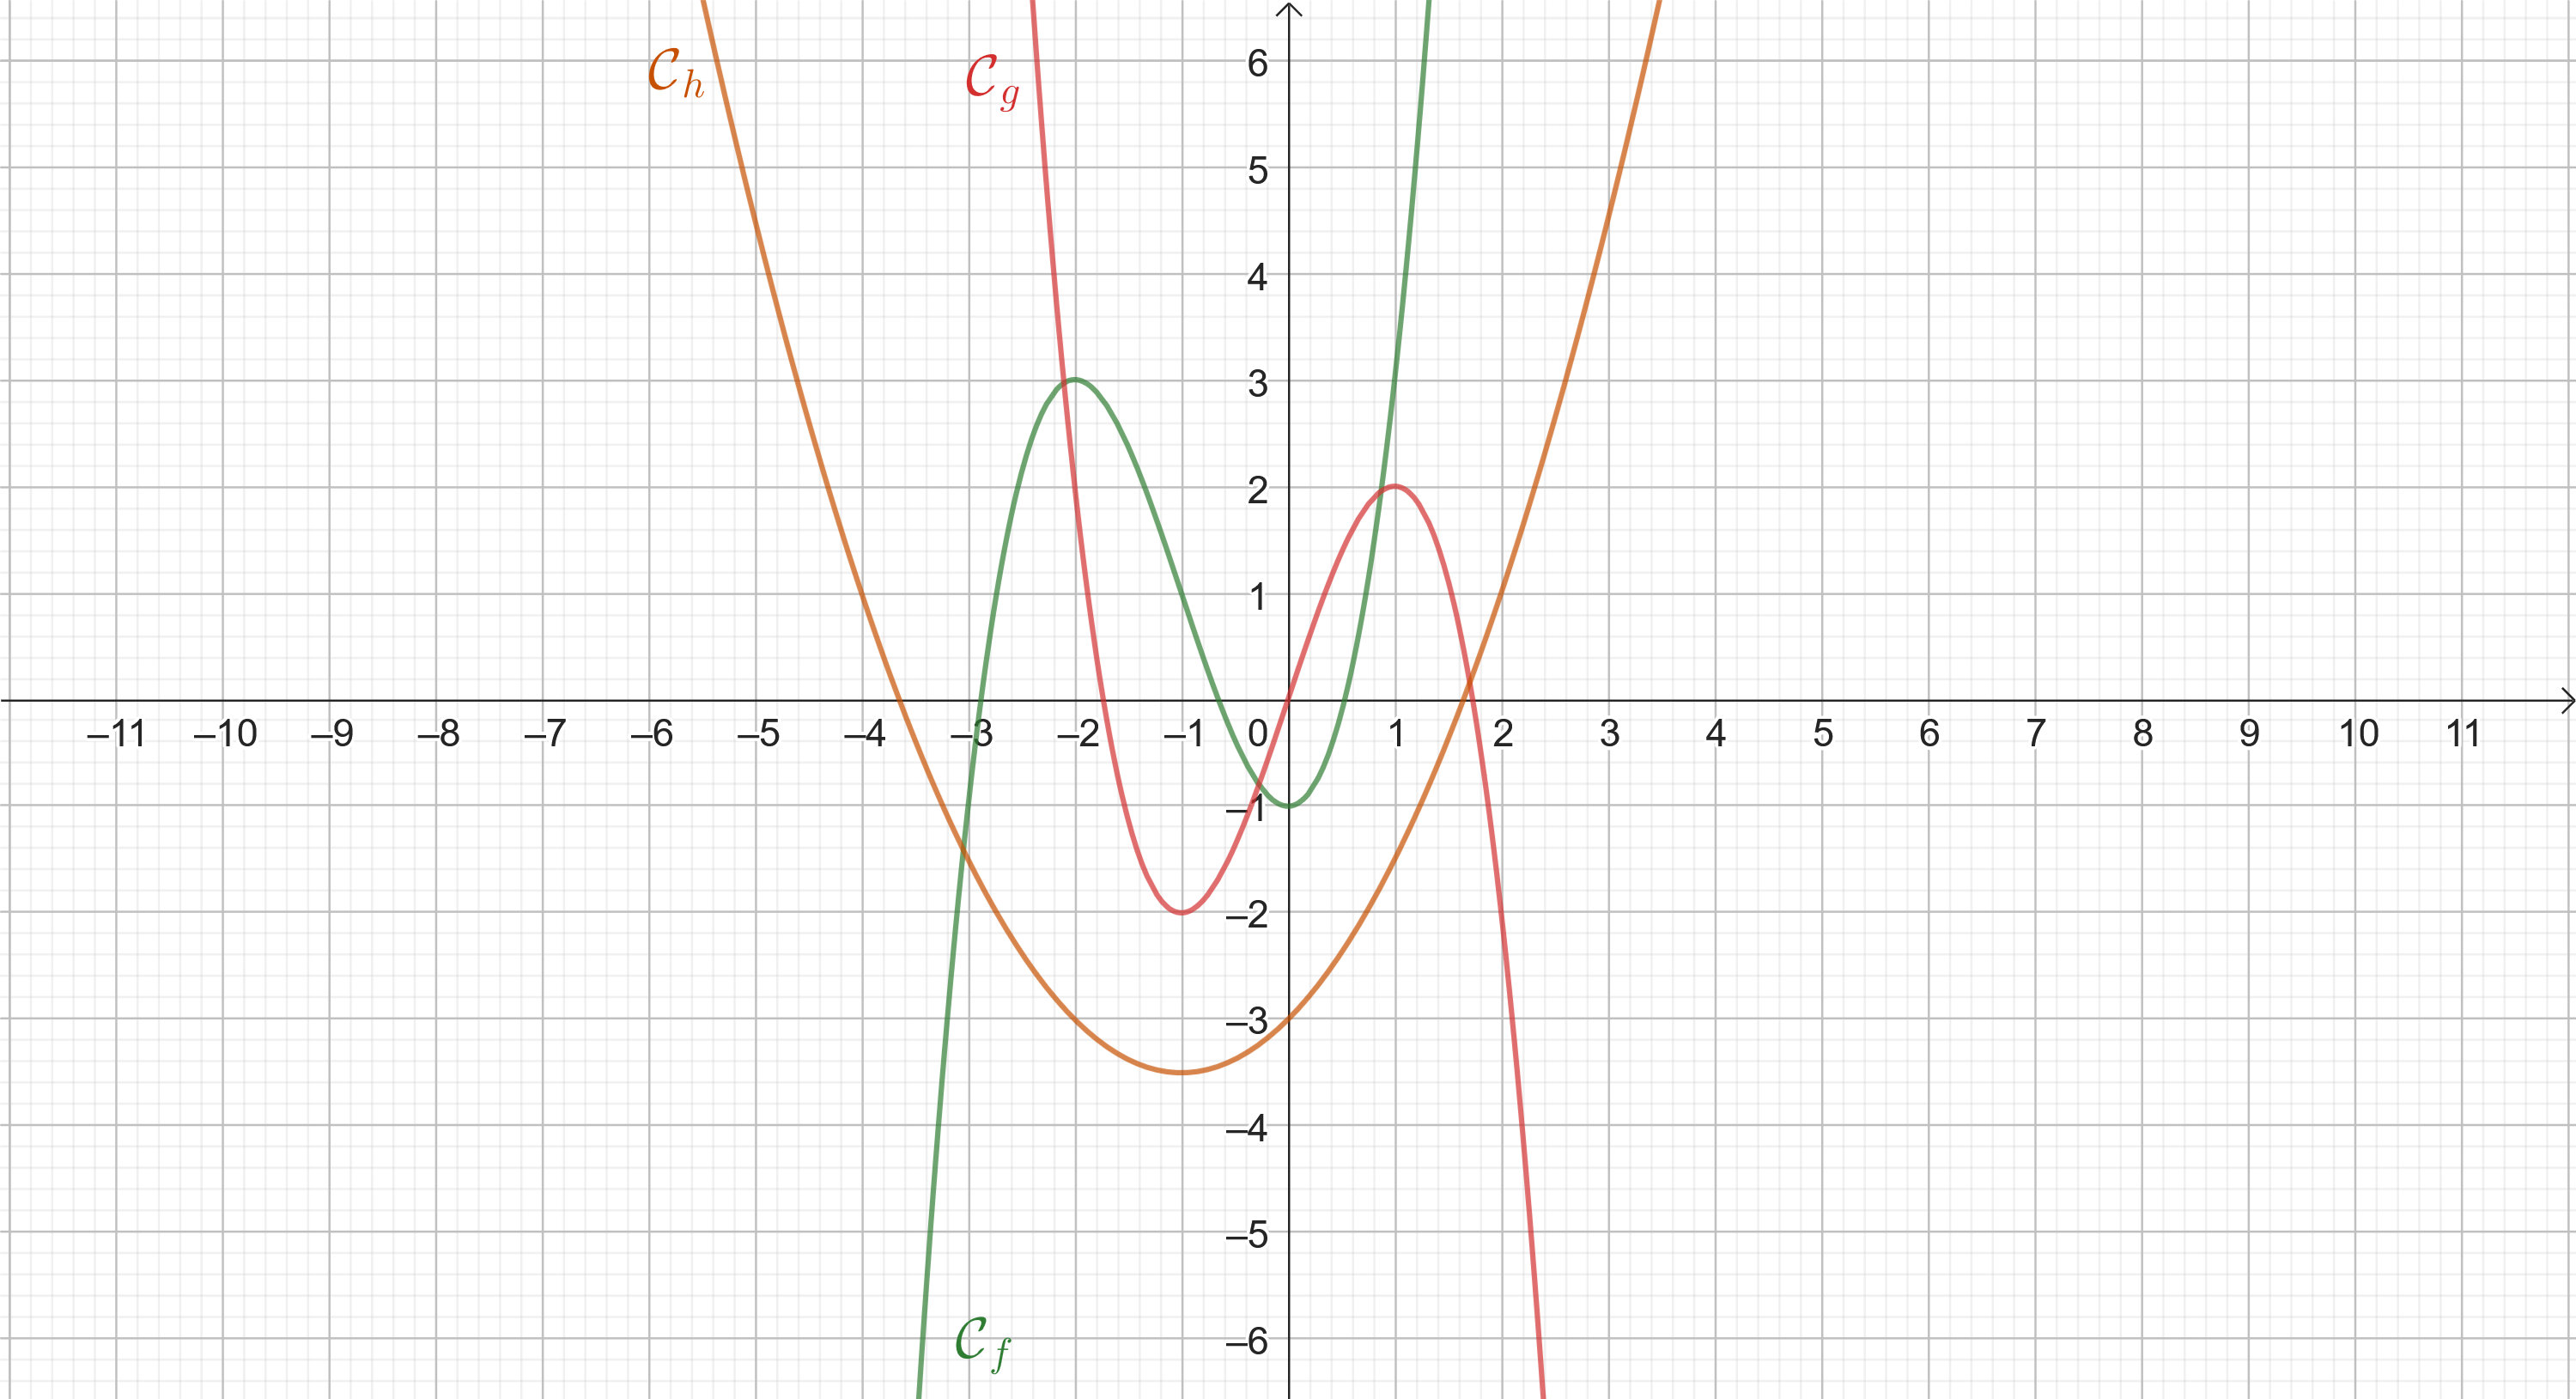
\includegraphics[width=\textwidth]{Courbes.png}
\end{center}
\section{Répondre aux questions suivantes par lecture graphique :}
\begin{enumquestions}
\item Donner l'image de $0$ par la fonction $f$ : \answersline
\item Donner l'image de $-1$ par la fonction $g$ : \answersline
\item Donner l'image de $-4$ par la fonction $h$ : \answersline
\item Donner la valeur de $f(1)$ : \answersline
\item Donner la valeur de $g(-2)$ : \answersline
\item Donner \textsc{un} antécédent de $2$ par la fonction $g$ : \answersline
\item Donner \textsc{les} antécédents de $-2$ par la fonction $f$ : \answersline
\item Résoudre l'équation $h(x) = 1$ : \answersline
\item Combien $0$ a-t-il d'antécédents par la fonction $f$ ? : \answersline
\item Combien $-3$ a-t-il d'antécédents par la fonction $h$ ? : \answersline
\item Combien de solutions a l'équation $g(x)=-1$ : \answersline
\item Quelle fonction transforme $0$ en $0$ ? \answersline
\item Quelle fonction admet $1$ comme antécédent de $2$ ? \answersline
\item Quelle fonction admet $3$ antécédents de $1$ ? \answersline
\end{enumquestions}
\section{Tracer la courbe représentative d'une fonction $j$ vérifiant les critères suivants}
\begin{enumquestions}
\item L'image de $1$ par $j$ est $5$
\item $j(0) = 2$
\item Un antécédent de $-2$ par $j$ est $-2$, mais ce n'est pas le seul.
\item Le seul antécédent de $6$ est $-3$.
\end{enumquestions}
\end{document}